\section{Middleware}
\begin{itemize}
   \item struttura middleware (akka + websocket)
   \begin{itemize}
      \item Attore
      \begin{itemize}
         \item RealActor
         \item MockActor
      \end{itemize}
      \item Associazione tra corpo e mente (Attori + Eventbus) (name + type)
      \item WebSocket (messaggi sono solo "string")
   \end{itemize}
   \item URL di collegamento alle websocket (con aggiunta di parametri type + name)
   \item Vincoli
   \begin{itemize}
      \item Mente e corpo con lo stesso nome (case sensitive)
      \item Il contenuto principale dei messaggi scambiati tra le due entità deve iniziare con una lettera minuscola per rispettare la sintassi dei belief di Jason,
   \end{itemize}
\end{itemize}

\change[inline]{da sistemare}
\subsection{Struttura}

\begin{figure}[H]
\centering
\includegraphics[width=\textwidth]{figures/Middleware_reduced_structure.png}
\caption{Struttura interna del middleware}
\end{figure}

Synapsis è interamente realizzato utilizzando il framework Play, %illustrato nella sezione \ref{play}, 
le cui peculiarità sono la modularità e la distribuzione, raggiunte grazie all'utilizzo di Akka. Il sistema ad attori ha portato alla definizione di un'entità "copia" all'interno del middleware, strutturata allo stesso modo dell'entità "esterna" presente in parte su GE ed in parte su MAS.

\medskip

Questa soluzione ha semplificato concettualmente la gestione, da parte del middleware, delle entità esterne. Difatti, realizzando un attore che identifichi il corpo ed un attore che identifichi la mente è venuta meno la realizzazione di una componente logica per lo smistamento dei messaggi ricevuti dall'esterno. Ad esempio, quando un attore "mente" riceve un messaggio dall'esterno è consapevole che tale messaggio è stato generato ed inviato dall'entità "mente" esterna e, di conseguenza, è chiaro che il destinatario è l'attore "corpo" che, a sua volta, invia il messaggio all'entità "corpo" esterna.

\begin{figure}[H]
\centering
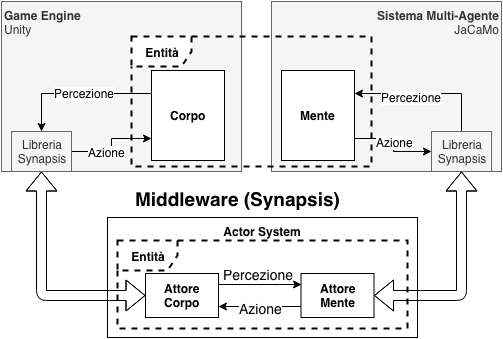
\includegraphics[width=\textwidth]{figures/Middleware_associazione_entita.png}
\caption{Associazione tra entità "esterna" ed "interna"}
\end{figure}

Lo schema riportato illustra il concetto precedentemente definito, in cui ad ogni entità esistente nei sistemi MAS e GE viene associata una coppia di attori "mente" e "corpo" all'interno del middleware.

\subsection{Collegamento tra attore e entità}

Il framework Play offre diverse modalità per rendere raggiungibile l'applicazione dall'esterno come, ad esempio, richieste HTTP sincrone, asincrone e WebSocket (WS). Queste ultime sono risultate le più adatte per effettuare il collegamento tra attore e entità, data la possibilità di instaurare una connessione duratura e bidirezionale.

\medskip

Con l'instaurazione di un collegamento WS, Play si occupa di inglobare il canale in un attore di sistema, rendendo possibile il suo utilizzo nel sistema ad attori e mettendo a disposizione dello sviluppatore il riferimento dell'attore appena creato. 
\smallskip
In Synapsis, questo riferimento viene passato all'effettivo attore che si occuperà di gestire i messaggi inviati dall'entità. Lo stesso procedimento viene eseguito per ogni connessione aperta, quindi, il rapporto tra numero di connessioni WS e attori "mente/corpo" è sempre di 1:1. \unsure{devo motivare la scelta del rapporto 1:1?} In caso di chiusura del canale WS, Play rimuove automaticamente l'attore creato in precedenza dal sistema.
\begin{figure}[H]
\centering
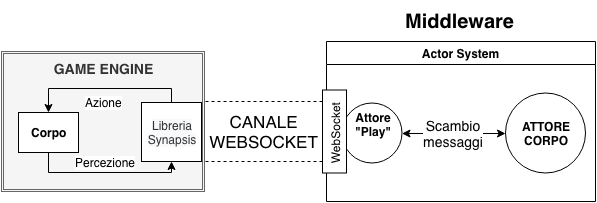
\includegraphics[width=\textwidth]{figures/Middleware_entita_attore.png}
\caption{Collegamento tra attore e entità}
\end{figure}

\improvement[inline]{Inserire e spiegare il link per collegarsi al middleware}

Url locale per collegarsi al middleware:
\begin{itemize}
    \item ws://localhost:9000\textbf{/synapsiservice/type/name}
\end{itemize}

\subsection{Collegamento tra attori mente e corpo} \label{soluzione_collegamento_attori}

All'intero del sistema ad attori non è possibile inviare messaggi senza avere il riferimento del destinatario. Questo aspetto ha rappresentato un problema per il collegamento interno tra attore "mente" e attore "corpo", dato che entrambi sono stati creati nel sistema ad attori successivamente all'instaurazione di un canale WS. Infatti, non è sicuro che l'entità "corpo" e l'entità "mente" si colleghino simultaneamente a Synapsis.

\medskip

EventBus\footnote{Classe presente nella libreria \href{https://doc.akka.io/docs/akka/current/event-bus.html}{Akka}}, a disposizione degli sviluppatori, permette di creare un sistema di notifiche broadcast, identificate da uno specifico argomento, a tutti gli attori registrati allo stesso tipo di argomento. All'interno del middleware è stato utilizzato per gestire il primo collegamento e la disconnessione tra attori della stessa entità. L'immagine sottostante rappresenta come avviene utilizzato l'EventBus.

\begin{figure}[H]
\centering
\includegraphics[width=\textwidth]{figures/EventBus.png}
\caption{Utilizzo EventBus per primo collegamento attori}
\end{figure}
\change[inline]{centrare il titolo della figura}

Di seguito viene illustrato un esempio di funzionamento in caso di aggiunta di un nuovo attore (corpo), ipotizzando che la controparte (mente) sia già presente all'interno del sistema:
\begin{enumerate}
    \item Il nuovo attore si registra agli argomenti \textit{"nuovo\_attore"} e \textit{"rimosso\_attore"};
    \item L'attore invia all'EventBus un messaggio all'argomento \textit{"nuovo\_attore"};
    \item L'EventBus notifica un messaggio a tutti i sottoscritti a quel determinato evento. Nel messaggio inviato viene allegato anche il riferimento all'attore creatore dell'evento;
    \item L'attore "mente" riceve il messaggio con il riferimento all'attore e notifica all'EventBus la propria presenza cosi da far ricevere il proprio riferimento all'attore "corpo" appena unito al sistema.
\end{enumerate}
